\iffalse
\documentclass[journal,12pt,twocolumn]{IEEEtran}
\usepackage{setspace}
\usepackage{gensymb}
\usepackage{xcolor}
\usepackage{caption}
%\usepackage{subcaption}
%\doublespacing
\singlespacing
\usepackage{siunitx}
%\usepackage{graphicx}
%\usepackage{amssymb}
%\usepackage{relsize}
\usepackage[cmex10]{amsmath}
\usepackage{mathtools}
%\usepackage{amsthm}
%\interdisplaylinepenalty=2500
%\savesymbol{iint}
%\usepackage{txfonts}
%\restoresymbol{TXF}{iint}
%\usepackage{wasysym}
\usepackage{hyperref}
\usepackage{amsthm}
\usepackage{mathrsfs}
\usepackage{txfonts}
\usepackage{stfloats}
\usepackage{cite}
\usepackage{cases}
\usepackage{subfig}
%\usepackage{xtab}
\usepackage{longtable}
\usepackage{multirow}
%\usepackage{algorithm}
%\usepackage{algpseudocode}
%\usepackage{enumerate}
\usepackage{enumitem}
\usepackage{mathtools}
%\usepackage{iithtlc}
%\usepackage[framemethod=tikz]{mdframed}
\usepackage{listings}
\usepackage{tikz}
\usetikzlibrary{shapes,arrows,positioning}
\usepackage{circuitikz}
\let\vec\mathbf


%\usepackage{stmaryrd}


%\usepackage{wasysym}
%\newcounter{MYtempeqncnt}
\DeclareMathOperator*{\Res}{Res}
%\renewcommand{\baselinestretch}{2}
\renewcommand\thesection{\arabic{section}}
\renewcommand\thesubsection{\thesection.\arabic{subsection}}
\renewcommand\thesubsubsection{\thesubsection.\arabic{subsubsection}}

\renewcommand\thesectiondis{\arabic{section}}
\renewcommand\thesubsectiondis{\thesectiondis.\arabic{subsection}}
\renewcommand\thesubsubsectiondis{\thesubsectiondis.\arabic{subsubsection}}

%\renewcommand{\labelenumi}{\textbf{\theenumi}}
%\renewcommand{\theenumi}{P.\arabic{enumi}}

% correct bad hyphenation here
\hyphenation{op-tical net-works semi-conduc-tor}

\lstset{
language=Python,
frame=single, 
breaklines=true,
columns=fullflexible
}



\begin{document}
%

\theoremstyle{definition}
\newtheorem{theorem}{Theorem}[section]
\newtheorem{problem}{Problem}
\newtheorem{proposition}{Proposition}[section]
\newtheorem{lemma}{Lemma}[section]
\newtheorem{corollary}[theorem]{Corollary}
\newtheorem{example}{Example}[section]
\newtheorem{definition}{Definition}[section]
%\newtheorem{algorithm}{Algorithm}[section]
%\newtheorem{cor}{Corollary}
\newcommand{\BEQA}{\begin{eqnarray}}
\newcommand{\EEQA}{\end{eqnarray}}
\newcommand{\define}{\stackrel{\triangle}{=}}
\newcommand{\myvec}[1]{\ensuremath{\begin{pmatrix}#1\end{pmatrix}}}
\newcommand{\mydet}[1]{\ensuremath{\begin{vmatrix}#1\end{vmatrix}}}

\bibliographystyle{IEEEtran}
%\bibliographystyle{ieeetr}

\providecommand{\nCr}[2]{\,^{#1}C_{#2}} % nCr
\providecommand{\nPr}[2]{\,^{#1}P_{#2}} % nPr
\providecommand{\mbf}{\mathbf}
\providecommand{\pr}[1]{\ensuremath{\Pr\left(#1\right)}}
\providecommand{\qfunc}[1]{\ensuremath{Q\left(#1\right)}}
\providecommand{\sbrak}[1]{\ensuremath{{}\left[#1\right]}}
\providecommand{\lsbrak}[1]{\ensuremath{{}\left[#1\right.}}
\providecommand{\rsbrak}[1]{\ensuremath{{}\left.#1\right]}}
\providecommand{\brak}[1]{\ensuremath{\left(#1\right)}}
\providecommand{\lbrak}[1]{\ensuremath{\left(#1\right.}}
\providecommand{\rbrak}[1]{\ensuremath{\left.#1\right)}}
\providecommand{\cbrak}[1]{\ensuremath{\left\{#1\right\}}}
\providecommand{\lcbrak}[1]{\ensuremath{\left\{#1\right.}}
\providecommand{\rcbrak}[1]{\ensuremath{\left.#1\right\}}}
\theoremstyle{remark}
\newtheorem{rem}{Remark}
\newcommand{\sgn}{\mathop{\mathrm{sgn}}}
\providecommand{\abs}[1]{\left\vert#1\right\vert}
\providecommand{\res}[1]{\Res\displaylimits_{#1}} 
\providecommand{\norm}[1]{\lVert#1\rVert}
\providecommand{\mtx}[1]{\mathbf{#1}}
\providecommand{\mean}[1]{E\left[ #1 \right]}
\providecommand{\fourier}{\overset{\mathcal{F}}{ \rightleftharpoons}}
\providecommand{\ztrans}{\overset{\mathcal{Z}}{ \rightleftharpoons}}
\providecommand{\diff}[2]{\ensuremath{\frac{d{#1}}{d{#2}}}}
%\providecommand{\hilbert}{\overset{\mathcal{H}}{ \rightleftharpoons}}
\providecommand{\system}[1]{\overset{\mathcal{#1}}{\longleftrightarrow}}
	%\newcommand{\solution}[2]{\textbf{Solution:}{#1}}
\newcommand{\solution}{\noindent \textbf{Solution: }}
\providecommand{\dec}[2]{\ensuremath{\overset{#1}{\underset{#2}{\gtrless}}}}
\numberwithin{equation}{section}
%\numberwithin{equation}{subsection}
%\numberwithin{problem}{subsection}
%\numberwithin{definition}{subsection}
\makeatletter
\@addtoreset{figure}{problem}
\makeatother

\let\StandardTheFigure\thefigure
%\renewcommand{\thefigure}{\theproblem.\arabic{figure}}
\renewcommand{\thefigure}{\theproblem}
\renewcommand{\thefigure}{\arabic{section}.\arabic{figure}}
\makeatletter
\@addtoreset{figure}{section}
\makeatother

%\numberwithin{figure}{subsection}

\def\putbox#1#2#3{\makebox[0in][l]{\makebox[#1][l]{}\raisebox{\baselineskip}[0in][0in]{\raisebox{#2}[0in][0in]{#3}}}}
     \def\rightbox#1{\makebox[0in][r]{#1}}
     \def\centbox#1{\makebox[0in]{#1}}
     \def\topbox#1{\raisebox{-\baselineskip}[0in][0in]{#1}}
     \def\midbox#1{\raisebox{-0.5\baselineskip}[0in][0in]{#1}}

\vspace{3cm}

\title{ 
Circuits and Transforms
}

\author{Gautam Singh}

% make the title area
\maketitle

%\newpage

\tableofcontents

%\renewcommand{\thefigure}{\thesection.\theenumi}
%\renewcommand{\thetable}{\thesection.\theenumi}

\renewcommand{\thefigure}{\theenumi}
\renewcommand{\thetable}{\theenumi}

%\renewcommand{\theequation}{\thesection}


\bigskip

\begin{abstract}
This manual provides a simple introduction to Transforms
\end{abstract}
\fi

\section{Definitions}
\begin{enumerate}[label=\arabic*.,ref=\thesection.\theenumi]
\numberwithin{equation}{enumi}
\numberwithin{figure}{enumi}
\item The unit step function is defined as
\begin{align}
u(t) =
\begin{cases}
1 & t > 0
\\
	\frac{1}{2} & t = 0
\\
0 & t < 0
\end{cases}
\end{align}
\item The Laplace transform of $g(t)$ is defined as 
\begin{align}
	G(s) = \int_{-\infty}^{\infty} g(t) e^{-st}\, dt
\end{align}
 \end{enumerate}

 \section{Laplace Transform}
In the circuit
			in Fig. \ref{fig:cktsig/ckt},
the switch $S$ is connected to position $P$ for a long time so that the charge on the capacitor
	becomes $q_1 \, \mu C$. Then $S$ is switched to position $Q$.  After a long time, the charge on the capacitor is
		$q_2 \, \mu C$.  Use variables $R_1, R_2, C_0$ for 
the passive elements.	
		\begin{figure}[!ht]
			\centering
			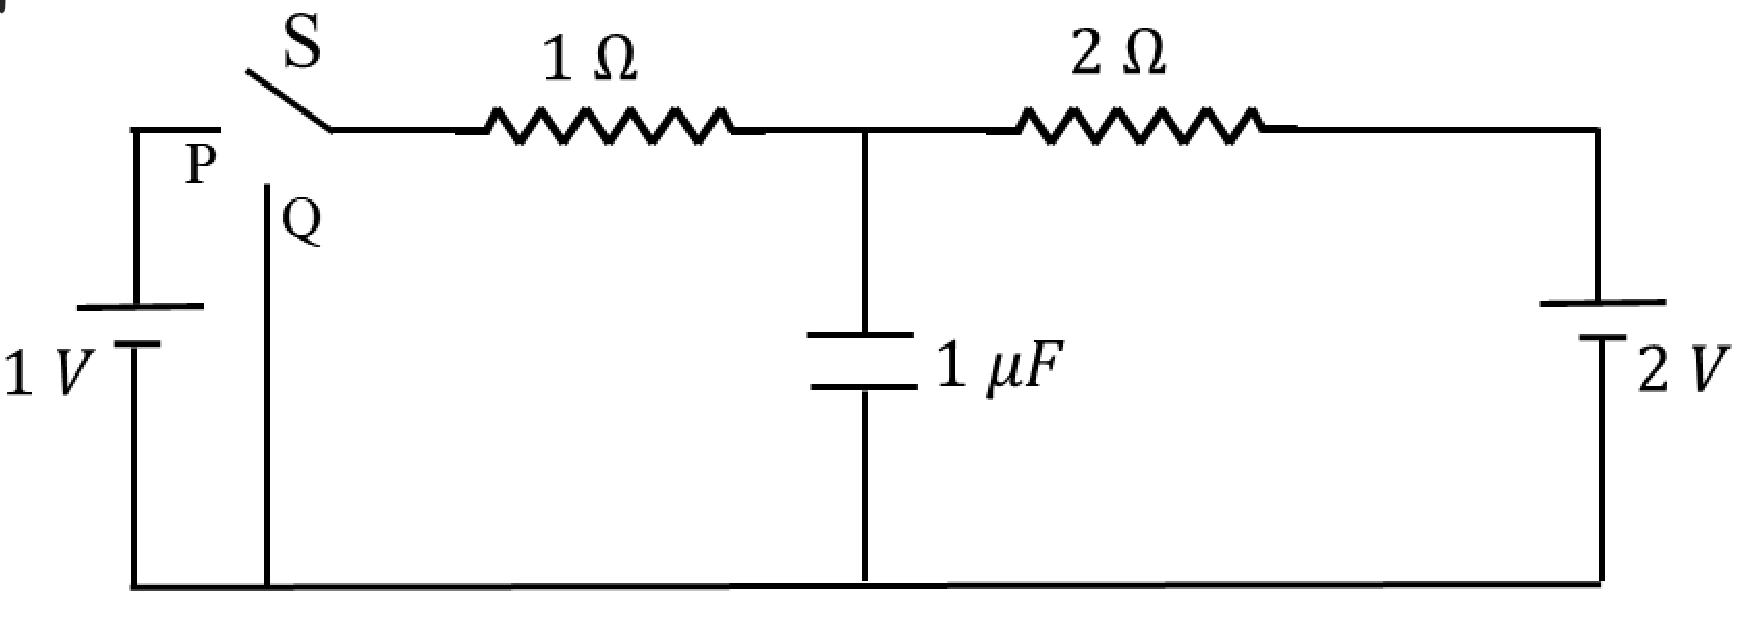
\includegraphics[width=\columnwidth]{cktsig/figs/ckt.jpg}
			\caption{}
			\label{fig:cktsig/ckt}
\end{figure}
\begin{enumerate}[label=\arabic*.,ref=\thesection.\theenumi]
\numberwithin{equation}{enumi}
\numberwithin{figure}{enumi}
\item Draw the circuit in position $P$.
	\\
		\solution See Fig. 
    \ref{fig:cktsig/ckt-q1}
drawn using the code in 
		\begin{lstlisting}
			cktsig/figs/ckt-q1.tex
		\end{lstlisting}
\begin{figure}[!h]
	\centering
	    \begin{circuitikz} \draw
        (0,0) to[battery1, l=1 $V$, invert] (0,2)
        -- (0.5,2) node[label={above:P}] {}
        to[R, l^=$1 \Omega$, *-*] (3,2) 
        node[label={above:X}] {}
        to[R, l^=$2 \Omega$] (5.5,2)
        to[battery1, l=2 $V$] (5.5,0)
        -- (0,0)
        (3,2) to[C, l=1 ${\mu}F$] (3,0) 
        -- (3,-0.5) node[ground, label={right:G}] {};
    \end{circuitikz}

    \caption{}
    \label{fig:cktsig/ckt-q1}
\end{figure}
\item Simulate the circuit in 
    Fig. \ref{fig:cktsig/ckt-q1}
using ngspice.
\\
\solution The following ngspice script  simulates the given circuit.
\begin{lstlisting}
ngspice codes/2_7.cir
\end{lstlisting}
\item Find $q_1$ in Fig. 
\ref{fig:cktsig/sckt-q1-steady}.
\begin{figure}[!htb]
	\centering
	    \begin{circuitikz} 
    \ctikzset{resistor = european}
    \draw
    (0,0) to[battery1, invert, l = $ V_1$] (0,3)
    node[label={above:P}] {}
    to[R, l^=$R_1$, *-*] (3,3) 
    node[label={above:X}] {}
    to[R, l^=$R_2$] (5.5,3)
    to[battery1, l= $V_2$] (5.5,0)
    -- (0,0)
   % (3,3) to[R, l=$\frac{1}{sC_0}$] (3,0) 
    (3,0) 
    -- (3,-0.5) node[ground, label={right:G}] {};
    \end{circuitikz}

\caption{}
\label{fig:cktsig/sckt-q1-steady}
\end{figure}
\\
\solution Assuming the circuit to be grounded at G and the relative potential at point
X to be $V$, we use KCL at X and get
\begin{align}
	\frac{V - V_1}{R_1} + \frac{V - V_2}{R_2} &= 0 \\
	\\
	\implies V = \frac{V_1R_2 + V_2R_1}{R_1+R_2}&=
      \SI[parse-numbers=false]{\frac{4}{3}}{\V}
\end{align}
upon substituting numerical values.
Hence,
\begin{align}
    q_1 = CV = 
	  C\frac{\brak{V_1R_2 + V_2R_1}}{R_1+R_2}&=
     \SI[parse-numbers=false]{\frac{4}{3}}{\micro\coulomb}
\end{align}
\item Show that the Laplace transform of $u(t)$ is $\frac{1}{s}$ and find the ROC.
	\\
\solution We have,
\begin{align}
	u(t) &\system{L} \int_{0}^{\infty}u(t)e^{-st}dt \\
         &= \int_{0}^{0}\frac{1}{2}e^{-st}dt + \int_{0}^{\infty}e^{-st}dt \\
         &= \frac{1}{s}, \quad \Re{(s)} > 0
         \label{eq:cktsig/L-u}
\end{align}
\item Now consider the following resistive circuit 
in Fig. 
\ref{fig:cktsig/sckt-q1-s}
	transformed from 
Fig. \ref{fig:cktsig/ckt}
		where 
		\begin{align}
			v_1(t) = u(t) \system{L} V_1(s) = \frac{1}{s}
			\\
			v_2(t) = 2u(t) \system{L} V_2(s) = \frac{2}{s}
		\end{align}
		Find the voltage across the capacitor $V_{C_0}(s)$.
\begin{figure}[!htb]
	\centering
	    \begin{circuitikz} 
    \ctikzset{resistor = european}
    \draw
	    (0,0) to[battery1, invert, l = $V_1(s)$] (0,3)
    node[label={above:P}] {}
    to[R, l^=$R_1$, *-*] (3,3) 
    node[label={above:X}] {}
    to[R, l^=$R_2$] (5.5,3)
	    to[battery1, l= $ V_2(s)$] (5.5,0)
    -- (0,0)
    (3,3) to[R, l=$\frac{1}{sC_0}$] (3,0) 
    -- (3,-0.5) node[ground, label={right:G}] {};
    \end{circuitikz}

\caption{}
\label{fig:cktsig/sckt-q1-s}
\end{figure}
\\
\solution Applying KCL at $X$,
\begin{align}
	\frac{V(s) - \frac{1}{s}}{R_1} + \frac{V(s) - \frac{2}{s}}{R_2} + sC_0V(s) &= 0 \\
	\implies	V(s)\brak{\frac{1}{R_1} + \frac{1}{R_2} + sC_0} &= \frac{1}{s}\brak{\frac{1}{R_1} + \frac{2}{R_2}} \\
\implies	V(s) &= \frac{\frac{1}{R_1} + \frac{2}{R_2}}{s\brak{\frac{1}{R_1} + \frac{1}{R_2} + sC_0}} \\
    &= \frac{\frac{1}{R_1} + \frac{2}{R_2}}{\frac{1}{R_1} + \frac{1}{R_2}}\brak{\frac{1}{s} - \frac{1}{\frac{1}{C_0}\brak{\frac{1}{R_1} + \frac{1}{R_2}} + s}} 
    \label{eq:cktsig/V-s}
\end{align}
\item Show that 
		\begin{align}
			e^{-at}u(t) \system{L} \frac{1}{s+a}, \quad a > 0
			\label{eq:cktsig-exp}
		\end{align}
		and find the ROC.
		\\
\solution Note that by substituting $s := s + a$ in \eqref{eq:cktsig/L-u}, and considering
$a \in \mathbb{R}$,
\begin{align}
	e^{-at}u(t) &\system{L} \int_{0}^{\infty}u(t)e^{-(s + a)t}dt \\
                &= \frac{1}{s + a}, \quad \Re{(s)} > -a
                \label{eq:cktsig/L-u-shift}
\end{align}
\item Find $v_{C_0}(t)$.  
	\\
\solution Taking the inverse Laplace transform in \eqref{eq:cktsig/V-s},
\begin{align}
	V(s) \system{L}{-1} \frac{2R_1 + R_2}{R_1 + R_2}u(t)\brak{1 - e^{-\brak{\frac{1}{R_1} + \frac{1}{R_2}}\frac{t}{C_0}}} 
%	\\
%    &= \frac{4}{3}\brak{1 - e^{-\brak{1.5 \times 10^6}t}}u(t)
\end{align}
from 
			\eqref{eq:cktsig-exp}.
\item Verify your result numerically. 
	\\
	\solution 
The following python code 
\iffalse
\begin{lstlisting}
python3 codes/2_6.py
\end{lstlisting}
    \ref{fig:cktsig/v1-t}.
\begin{figure}[!htb]
	\centering
    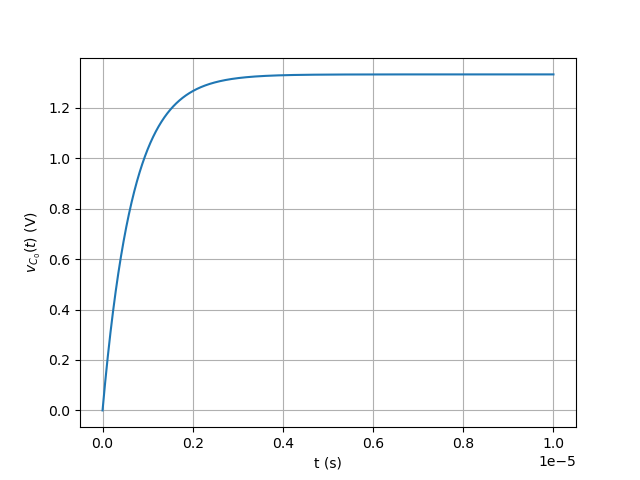
\includegraphics[width=\columnwidth]{cktsig/figs/2_6.png}
    \caption{$v_{C_0}(t)$ before the switch is flipped}
    \label{fig:cktsig/v1-t}
\end{figure}
Plot using python. 
\\
\solution The following ngspice script  simulates the given circuit and the generated output is shown in Fig. 
\fi
 plots the graph in Fig. 
    \ref{fig:cktsig/v1-sim-t}
\begin{lstlisting}
python3 codes/2_6-sim.py
\end{lstlisting}
\begin{figure}[!htb]
	\centering
    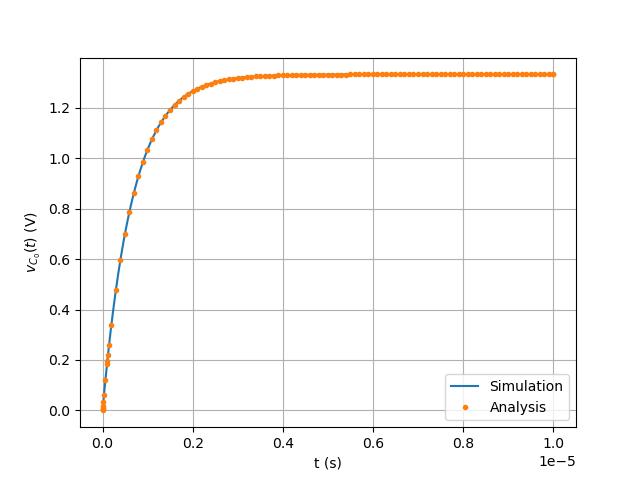
\includegraphics[width=\columnwidth]{cktsig/figs/2_6-sim.png}
    \caption{$v_{C_0}(t)$ simulation}
    \label{fig:cktsig/v1-sim-t}
\end{figure}
\end{enumerate}

\section{Initial Conditions}
\begin{enumerate}[label=\arabic*.,ref=\thesection.\theenumi]
\numberwithin{equation}{enumi}
\item Draw the equivalent circuit when the switch is at Q. 
	\\
		\solution See Fig. 
\ref{fig:cktsig/ckt-q2}.
below.
\begin{figure}[!htb]
	    \centering
	    \begin{circuitikz} \draw
    (0,0) -- (0,2)
    node[label={above:Q}] {}
    to[R, l^=$1 \Omega$, *-*] (3,2) 
    node[label={above:X}] {}
    to[R, l^=$2 \Omega$] (5.5,2)
    to[battery1, l=2 $V$] (5.5,0)
    -- (0,0)
    (3,2) to[C, l=1 ${\mu}F$] (3,0) 
    -- (3,-0.5) node[ground, label={right:G}] {};
    \end{circuitikz}

\caption{}
\label{fig:cktsig/ckt-q2}
\end{figure}
\item Find $q_2$ in Fig. 
    \ref{fig:cktsig/ckt-q2-steady}.
\\
\solution The equivalent circuit at steady state when the switch is at Q is shown
in Fig.
    \ref{fig:cktsig/ckt-q2-steady}.
\begin{figure}[!h]
	\centering
	    \begin{circuitikz} 
    \ctikzset{resistor = european}
    \draw
    (0,0) -- (0,3)
    node[label={above:P}] {}
    to[R, l^=$R_1$, *-*] (3,3) 
    node[label={above:X}] {}
    to[R, l^=$R_2$] (5.5,3)
    to[battery1, l= $V_2$] (5.5,0)
    -- (0,0)
   % (3,3) to[R, l=$\frac{1}{sC_0}$] (3,0) 
    (3,0) 
    -- (3,-0.5) node[ground, label={right:G}] {};
    \end{circuitikz}

    \caption{}
    \label{fig:cktsig/ckt-q2-steady}
\end{figure}
Since the capacitor behaves as an open circuit, we use voltage division at $X$ to obtain
\begin{align}
	V = V_1\frac{R_1}{R_1+R_2}=\SI[parse-numbers=false]{\frac{2}{3}}{\V}
\end{align}                                         
upon substituting numerical values.  Hence, 
\begin{align}
q_2 = CV = \SI[parse-numbers=false]{\frac{2}{3}}{\micro\coulomb}.
\end{align}

\item Draw the equivalent $s$-domain resistive circuit when $S$ 
is switched to position Q. 
\\
See Fig. 
\ref{fig:cktsig/sckt-q2-s}.
\begin{figure}[!htb]
	\centering
	    \begin{circuitikz} 
    \ctikzset{resistor = european}
    \draw
    (0,0) -- (0,3)
    node[label={above:Q}] {}
    to[R, l^=$R_1$, *-*] (3,3) 
    node[label={above:X}] {}
    to[R, l^=$R_2$] (5.5,3)
    to[battery1, l= $\frac{2}{s} V$] (5.5,0)
    -- (0,0)
    (3,3) to[battery1, l=$\frac{4}{3s} V$] (3,2) to[R, l=$\frac{1}{sC_0}$] (3,0) 
    -- (3,-0.5) node[ground, label={right:G}] {};
    \end{circuitikz}

\caption{}
\label{fig:cktsig/sckt-q2-s}
\end{figure}
\item $V_{C_0}(s)$ = ?  
\\
\solution Using KCL at node $X$ in Fig.
\ref{fig:cktsig/sckt-q2-s},
\begin{align}
	\frac{V(s) - 0}{R_1} + \frac{V(s) - \frac{2}{s}}{R_2} + sC_0\brak{V(s) - \frac{4}{3s}} = 0 \\
\implies V_{C_0}(s) = \frac{\frac{2}{sR_2} + \frac{4C_0}{3}}{\frac{1}{R_1} + \frac{2}{R_2} + sC_0}
\label{eq:cktsig/v2-s}
\end{align}
\item $v_{C_0}(t)$ = ? 
\\
\solution From \eqref{eq:cktsig/v2-s}, using partial fractions, 
\begin{align}
    V_{C_0}(s) = \frac{4}{3}\brak{\frac{1}{\frac{1}{C_0}\brak{\frac{1}{R_1} + \frac{1}{R_2}}+s}} 
    + \frac{2}{R_2\brak{\frac{1}{R_1} +\frac{1}{R_2}}}\brak{\frac{1}{s} - \frac{1}{\frac{1}{C_0}\brak{\frac{1}{R_1} + \frac{1}{R_2}} + s}}
\end{align}
Taking the inverse Laplace Transform,
\begin{align}
    v_{C_0}(t) = \frac{4}{3}e^{-\brak{\frac{1}{R_1} + \frac{1}{R_2}}\frac{t}{C_0}}u(t)  
    + \frac{2}{R_2\brak{\frac{1}{R_1}+\frac{1}{R_2}}}\brak{1 - e^{-\brak{\frac{1}{R_1} + \frac{1}{R_2}}\frac{t}{C_0}}}u(t)
\end{align}
			from \eqref{eq:cktsig-exp}.
		\item Verify your result numerically.
			\\
			\solution
Substituting numerical values, 
\begin{align}
    v_{C_0}(t) = \frac{2}{3}\brak{1 +e^{-\brak{1.5 \times 10^6}t}}u(t)
    \label{eq:cktsig/v2-t}
\end{align}
This is verified by the following  code that plots 
Fig.
    \ref{fig:cktsig/v2-t} using ngspice and python.
\begin{lstlisting}
python3 codes/3_4-sim.py
\end{lstlisting}
\begin{figure}[!htb]
	\centering
    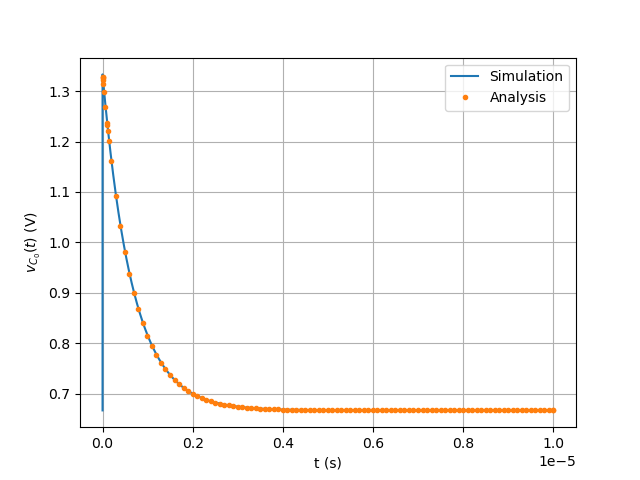
\includegraphics[width=\columnwidth]{cktsig/figs/3_4.png}
    \caption{$v_{C_0}(t)$ after the switch is flipped}
    \label{fig:cktsig/v2-t}
\end{figure}
\item Find $v_{C_0}(0-), v_{C_0}(0+)$ and  $v_{C_0}(\infty) $. 
\\
\solution From the initial conditions,
\begin{align}
    v_{C_0}(0-) = \frac{q_1}{C_0} = \SI[parse-numbers=false]{\frac{4}{3}}{\V}
\end{align}
Using \eqref{eq:cktsig/v2-t},
\begin{align}
    v_{C_0}(0+) &= \lim_{t \to 0+}v_{C_0}(t) = \SI[parse-numbers=false]{\frac{4}{3}}{\V} \\
    v_{C_0}(\infty) &= \lim_{t \to \infty}v_{C_0}(t) = \SI[parse-numbers=false]{\frac{2}{3}}{\V}
\end{align}

\end{enumerate}
\section{Bilinear Transform}
\begin{enumerate}[label=\arabic*.,ref=\thesection.\theenumi]
\numberwithin{equation}{enumi}
\item Formulate the differential equation for Fig. \ref{fig:cktsig/bilinear/ckt}.
	
\begin{figure}[!htb]
    \begin{center}
	        \begin{circuitikz}
        \draw (0,3) to[C, l=$C_0$, i = $i$] (0,0) -- (3,0)
        to[battery1, l=$V$, invert] (3,3) to[R, l^=$R_2$] (0,3);
    \end{circuitikz}

    \end{center}
\caption{}
\label{fig:cktsig/bilinear/ckt}
\end{figure}

\solution
Applying KVL on the loop,
\begin{align}
    V - iR_2 - \frac{1}{C_0}\int_0^tidt &= 0
    \label{eq:cktsig/bilinear/kvl}
\end{align}
where $i(0) = 0$, $V_C(0) = 0$. Denote by $V_C$ the voltage at the capacitor.
Then,
\begin{align}
    i = C\frac{dV_C}{dt}
    \label{eq:cktsig/bilinear/i-V}
\end{align}
and therefore using \eqref{eq:cktsig/bilinear/i-V} in \eqref{eq:cktsig/bilinear/kvl}, we get the differential equation
\begin{align}
    V - \tau\frac{dV_C}{dt} - V_C = 0
    \label{eq:cktsig/bilinear/diff-eqn}
\end{align}
where $\tau \triangleq R_2C_0$ is the time constant of the circuit.

\item Fig. \ref{fig:cktsig/bilinear/ckt} is transformed to 
Fig. \ref{fig:cktsig/bilinear/sckt} in the $s$ domain.
		Find  the {\em system transfer function}
\begin{align}
	H(s) = \frac{V(s)}{V_c(s)}
\end{align}
%considering the output voltage at the capacitor.
\begin{figure}[!htb]
    \begin{center}
	            \begin{circuitikz} 
    \ctikzset{resistor = european}
    \draw (0,3) to[R, l=$\frac{1}{sC_0}$] (0,0) 
    -- (3,0) to[battery1, l=$V(s)$, invert] (3,3) to[R, l^=$R_2$] (0,3);
    \end{circuitikz}

    \end{center}
\caption{}
\label{fig:cktsig/bilinear/sckt}
\end{figure}
\solution 
Using the voltage division formula, the voltage across 
the capacitor is given by
\begin{align}
    V_C(s) &= V(s)\frac{\frac{1}{sC}}{\frac{1}{sC} + R} 
           = V(s)\frac{1}{1 + sCR}
           \label{eq:cktsig/bilinear/vcs} \\
	\implies H(s) &= \frac{V_C(s)}{V(s)} = \frac{1}{1 + sCR}
    \label{eq:cktsig/bilinear/hs}
\end{align}
\item Plot $\abs{H(\j\omega}$. What kind of filter is it?
	\\
\solution 
\iffalse
		The Python code \texttt{codes/1\_3.py} plots $H(s)$.
\begin{figure}[!ht]
    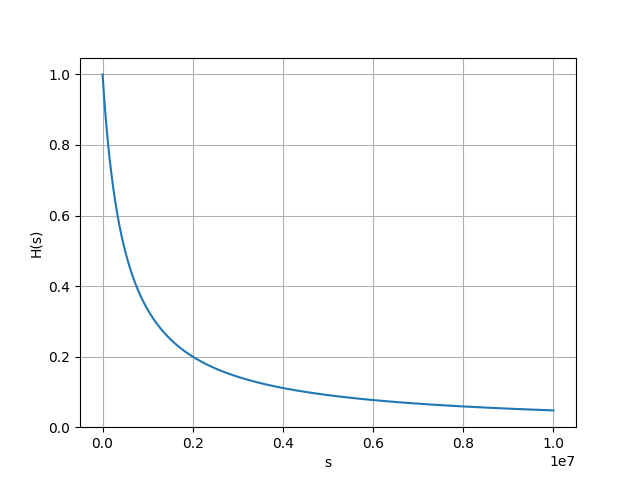
\includegraphics[width=\columnwidth]{cktsig/figs/1_3.png}
    \caption{Plot of $H(s)$.}
    \label{fig:cktsig/bilinear/hs}
\end{figure}
Clearly, $H(s)$ is a low-pass filter.
\fi
\item Using trapezoidal rule for integration, formulate 
    \eqref{eq:cktsig/bilinear/diff-eqn}
as a
difference
equation by considering 
\begin{align}
	V_C(n) = V_C(t)\vert_{t=n}
\end{align}
\solution Integrating \eqref{eq:cktsig/bilinear/diff-eqn} between limits $n-1$ to $n$ 
and applying the trapezoidal formula,
\begin{align}
    \frac{V_C\brak{n} + V_C\brak{n-1}}{2} + \tau\brak{V_C\brak{n}-V_C\brak{n-1}} 
    = \frac{V(n)+V(n-1)}{2}
    \\
	\implies 
	V_C\brak{n} \brak{\frac{ 1}{2}+ \tau } + V_C\brak{n-1}\brak{\frac{ 1}{2}- \tau} 
    = \frac{V(n)+V(n-1)}{2}
    \label{eq:cktsig/bilinear/difference-eqn}
\end{align}
\item Find 
\begin{align}
H(z) =  \frac{V_C(z)}{V(z)}.
\end{align}
\solution Applying the Z-transform on both sides of \eqref{eq:cktsig/bilinear/difference-eqn},
\begin{align}
    V_C(z)\sbrak{(2\tau + 1) - z^{-1}(2\tau - 1)} = V(z)\brak{1 + z^{-1}}
\end{align}
Hence,
\begin{align}
    H(z) = \frac{1+z^{-1}}{\brak{2\tau+1}-\brak{2\tau-1}z^{-1}}
    \label{eq:cktsig/bilinear/Hz}
\end{align}
\item Is the system defined by 
    \eqref{eq:cktsig/bilinear/difference-eqn} stable?
    \\
    \solution 
From     \eqref{eq:cktsig/bilinear/Hz}, 
$H(z)$ has a pole at 
\begin{align}
z =\frac{2\tau-1}{2\tau+1} 
\end{align}
Since 
\begin{align}
\abs{\frac{2\tau-1}{2\tau+1}} < 1,
\end{align}
the ROC of $H(z)$ is $\abs{z} > 1$, which implies that \eqref{eq:cktsig/bilinear/difference-eqn} represents a stable system.
\item How can you obtain $H(z)$ from $H(s)$?
\\
\solution We use the bilinear transformation. Setting
\begin{align}
    s \triangleq \frac{2}{T}\frac{1 - z^{-1}}{1 + z^{-1}}
\end{align}
we get
\begin{align}
    H(z) = \frac{1}{1 + \frac{2\tau}{T}\frac{1-z^{-1}}{1+z^{-1}}}
\end{align}
Setting $T = 1$ gives \eqref{eq:cktsig/bilinear/Hz}.

\item Find $v_C(n)$. Verify using ngspice and the differential equation.

\solution Note that $v(n) = Vu(n)$. Thus,
\begin{align}
    V(z) = \frac{V}{1-z^{-1}}
\end{align}
Therefore,
\begin{align}
    V_C(z) &= H(z)V(z) \\
         &= \frac{TV\brak{1+z^{-1}}}{\brak{1-z^{-1}}\brak{\brak{2\tau+T}-\brak{2\tau-T}z^{-1}}} \\
         &= \frac{V\brak{1+z^{-1}}}{2}\sum_{k=-\infty}^{\infty}\brak{1-p^k}u(k)z^{-k}
\end{align}
where $p \triangleq \frac{2\tau-T}{2\tau+T}$. Thus,
\begin{align}
    &v_C(n) = \nonumber \\
    &\begin{cases}
        \frac{V}{2}\sbrak{u(n)\brak{1-p^n}+u(n-1)\brak{1-p^{n-1}}} & n > 0 \\
        0 & n \le 0
    \end{cases}
    \label{eq:cktsig/bilinear/vn}
\end{align}
We take $T = 10^{-7}$ as the
sampling interval. The python code \texttt{codes/1\_7.py} verifies
these equalities.
\begin{figure}
    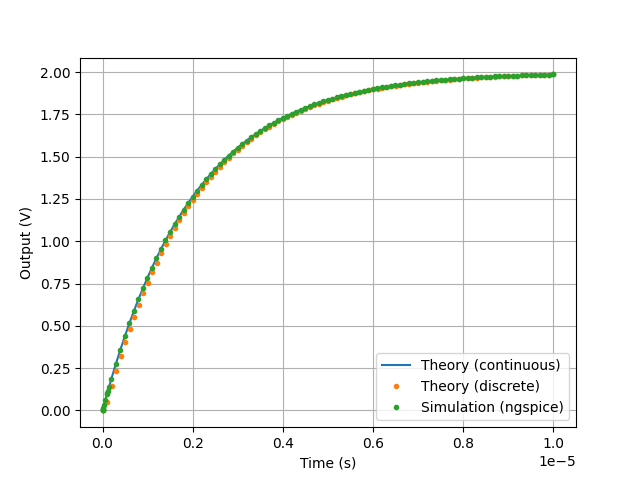
\includegraphics[width=\columnwidth]{cktsig/figs/1_7.png}
    \caption{Representation of output across $C$.}
    \label{fig:cktsig/bilinear/vc}
\end{figure}
\end{enumerate}
\iffalse
\section{Bilinear Transform}
\begin{enumerate}[label=\arabic*.,ref=\thesection.\theenumi]
\numberwithin{equation}{section}
\item In Fig. \ref{fig:cktsig/bilinear/cktsig/ckt}, consider the case when $S$ is switched to 
	$Q$ right in the beginning. Formulate the differential equation for $v_{C_0}(t)$.
\\
\solution The equivalent time domain circuit is available in Fig. 
\ref{fig:cktsig/bilinear/cktsig/tckt-q4}.
%	
\begin{figure}[!htb]
	\centering
    \begin{circuitikz} 
    \draw
    (0,0) -- (0,3)
    node[label={above:Q}] {}
    to[R, l^=$R_1$, *-*, i = $i_1$] (3,3) 
    node[label={above:X}] {}
    to[R, l^=$R_2$, i = $i_3$] (5.5,3)
    to[battery1, l= $V_2$] (5.5,0)
    -- (0,0)
    (3,3) to[C, l=$C_0$, i = $i_2$] (3,0) ;
    \end{circuitikz}

    \centering
\caption{}
\label{fig:cktsig/bilinear/cktsig/tckt-q4}
\end{figure}
%
Applying KCL and KVL,
\begin{align}
    &i_1 = i_2 + i_3 \\
    &i_1R_1 + \frac{1}{C_0}\int_0^ti_2\, dt = 0 \\
    &i_3R_2 + 2 - \frac{1}{C_0}\int_0^ti_2\, dt = 0
\end{align}
Differentiating the above equations,
\begin{align}
    &\diff{i_1}{t} = \diff{i_2}{t} + \diff{i_3}{t} \label{eq:cktsig/bilinear/cktsig/diff1}\\
    &R_1\diff{i_1}{t} + \frac{i_2}{C_0} = 0 \label{eq:cktsig/bilinear/cktsig/diff2}\\
    &R_2\diff{i_3}{t} - \frac{i_2}{C_0} = 0 \label{eq:cktsig/bilinear/cktsig/diff3}
\end{align}
Using \eqref{eq:cktsig/bilinear/cktsig/diff1} and \eqref{eq:cktsig/bilinear/cktsig/diff3} in \eqref{eq:cktsig/bilinear/cktsig/diff2},
\begin{align}
    &R_1\brak{\diff{i_2}{t} + \diff{i_3}{t}} + \frac{i_2}{C_0} = 0 \\
    &R_1\diff{i_2}{t} + \brak{1 + \frac{R_1}{R_2}}\frac{i_2}{C_0} = 0 \\
    &\diff{i_2}{t} + \brak{\frac{1}{R_1} + \frac{1}{R_2}}\frac{i_2}{C_0} = 0 \\
    &\diff{i_2}{t} + \frac{i_2}{\tau} = 0
    \label{eq:cktsig/bilinear/cktsig/diff-eqn-init}
\end{align}
where $\tau = \frac{C_0R_1R_2}{R_1 + R_2}$ is the RC time 
constant of the circuit. Note that $i_2(0) = \frac{V_2}{R_2}$ A and 
$i_2 = C_0\diff{V}{t}$, where $V$ is the voltage of the capacitor. 
Hence, integrating \eqref{eq:cktsig/bilinear/cktsig/diff-eqn-init},
\begin{align}
    C_0\diff{V}{t} - \frac{V_2}{R_2} + \frac{C_0V}{\tau} &= 0 \\
    \implies \diff{V}{t} + \frac{V}{\tau} = \frac{V_2}{C_0R_2}
    \label{eq:cktsig/bilinear/cktsig/diff-eqn}
\end{align}
\item Find $H(s)$ considering the output voltage at the capacitor.

\solution Transforming Fig. \ref{fig:cktsig/bilinear/cktsig/tckt-q4} to the $s$-domain,

\begin{figure}[!htb]
    \begin{center}
    \begin{circuitikz} 
    \ctikzset{resistor = european}
    \draw
    (0,0) -- (0,3)
    node[label={above:Q}] {}
    to[R, l^=$R_1$, *-*] (3,3) 
    node[label={above:X}] {}
    to[R, l^=$R_2$] (5.5,3)
    to[battery1, l= $V_2(s)$] (5.5,0)
    -- (0,0)
    (3,3) to[R, l=$\frac{1}{sC_0}$] (3,0) 
    -- (3,-0.5) node[ground, label={right:G}] {};
    \end{circuitikz}
    \end{center}
\caption{}
\label{fig:cktsig/bilinear/cktsig/sckt-q4}
\end{figure}

Applying nodal analysis at X, and noting that 
$H(s) = \frac{V(s)}{V_2(s)}$,
\begin{align}
    &\frac{V}{R_1} + \frac{V}{\frac{1}{sC_0}} + \frac{V - V_2}{R_2} = 0 \\
    &H(s)\brak{\frac{1}{R_1} + \frac{1}{R_2} + sC_0} = \frac{1}{R_2} \\
    &H(s) = \frac{\frac{1}{R_2}}{\frac{1}{R_1} + \frac{1}{R_2} + sC_0}
    \label{eq:cktsig/bilinear/cktsig/Hs}
\end{align}
\item Plot $H(s)$. What kind of filter is it?

\solution The Python code \texttt{codes/4\_3.py} plots $H(s)$.
\begin{figure}[!ht]
    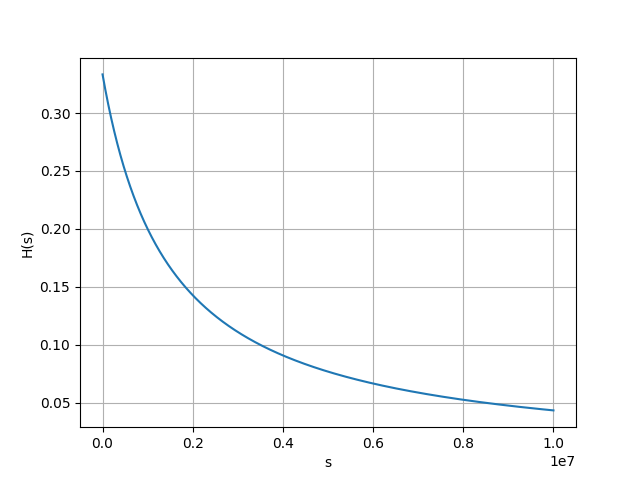
\includegraphics[width=\columnwidth]{cktsig/figs/4_3.png}
    \caption{Plot of $H(s)$.}
    \label{fig:cktsig/bilinear/cktsig/Hs}
\end{figure}
Clearly, $H(s)$ is a low-pass filter.
\item Using trapezoidal rule for integration, formulate the difference
equation by considering 
\begin{align}
	y(n) = y(t)\vert_{t=n}
\end{align}

\solution Integrating \eqref{eq:cktsig/bilinear/cktsig/diff-eqn} between limits $n$ to $n+1$ 
and applying the trapezoidal formula,
\begin{align}
    v(n+1) - v(n) + \frac{v(n) + v(n+1)}{2\tau} = \nonumber\\
    \frac{V_2\brak{u(n)+u(n+1)}}{C_0R_2} \\
    v(n)\brak{2\tau+1} + v(n-1)\brak{2\tau-1} = \nonumber\\ 
    \frac{V_2\tau\brak{u(n)+u(n-1)}}{C_0R_2}
    \label{eq:cktsig/bilinear/cktsig/difference-eqn}
\end{align}
for $n > 0$, where $v(0) = 0$.
\item Find $H(z)$.

\solution Note that for the input voltage, $v_i(n) = 2u(n)$ and
so, $V_i(z) = \frac{2}{1-z^{-1}}$. Applying the Z-transform
on both sides of \eqref{eq:cktsig/bilinear/cktsig/difference-eqn},
\begin{align}
    V(z)\sbrak{(2\tau + 1) - z^{-1}(2\tau - 1)} \nonumber \\
    = \frac{\tau\brak{1 + z^{-1}}V_i(z)}{C_0R_2}
\end{align}
Hence,
\begin{align}
    H(z) = \frac{\tau\brak{1+z^{-1}}}{C_0R_2\brak{\brak{2\tau+1}-\brak{2\tau-1}z^{-1}}}
    \label{eq:cktsig/bilinear/cktsig/Hz}
\end{align}
since $\abs{\frac{2\tau-1}{2\tau+1}} < 1$, the ROC is $\abs{z} > 1$.
\item How can you obtain $H(z)$ from $H(s)$?

\solution We use the bilinear transformation. Setting
\begin{align}
    s := \frac{2}{T}\frac{1 - z^{-1}}{1 + z^{-1}}
\end{align}
we get
\begin{align}
    H(z) &= \frac{\frac{1}{R_2}}{\frac{1}{R_1} + \frac{1}{R_2} + \frac{2C_0}{T}\frac{1 - z^{-1}}{1 + z^{-1}}} \\
         &= \frac{T\tau\brak{1+z^{-1}}}{C_0R_2\brak{\brak{2\tau+T}-\brak{2\tau-T}z^{-1}}}
\end{align}
Setting $T = 1$ gives \eqref{eq:cktsig/bilinear/cktsig/Hz}.

\item Find $v(n)$. Verify using ngspice and the differential equation.

\solution We have,
\begin{align}
    V(z) &= H(z)V_i(z) \\
         &= \frac{TV_2\tau\brak{1+z^{-1}}}{C_0R_2\brak{1-z^{-1}}\brak{\brak{2\tau+T}-\brak{2\tau-T}z^{-1}}} \\
         &= \frac{V_2\tau\brak{z+1}}{2C_0R_2}\sum_{k=-\infty}^{\infty}\brak{1-p^k}u(k)z^{-k}
\end{align}
where $p := \frac{2\tau-T}{2\tau+T}$. Thus,
\begin{align}
    v(n) = \frac{V_2\tau}{C_0R_2}\sbrak{u(n)\brak{1-p^n}+u(n+1)\brak{1-p^{n+1}}}
\end{align}
where $p := \frac{2\tau-1}{2\tau+1}$. We take $T = 10^{-7}$ as the
sampling interval. The python code \texttt{codes/4\_7.py} verifies
these equalities.
\begin{figure}
    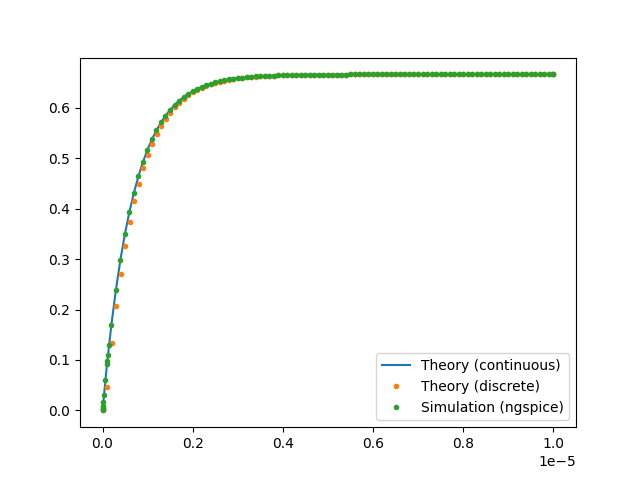
\includegraphics[width=\columnwidth]{cktsig/figs/4_7.png}
    \caption{Representation of output across $C_0$.}
    \label{fig:cktsig/bilinear/cktsig/vc0}
\end{figure}
\end{enumerate}
\fi
